\subsection{Regresión lineal}

La siguiente sección se centrara en la generación de modelos lineales para explicar la variable precio, tanto simples como compuestos, también se realizara una evaluación e interpretación de los resultados obtenidos mediante los mismos.\\
La idea sera predecir el precio de los productos base a ciertos predictores.

Se genero un nuevo data set de la variable precio, en donde se consolidaron algunas columnas nuevas, el data set propuesto para la siguiente investigación sera:


\begin{center}
 \begin{tabular}{||c c c c c c c||} 
 \hline
    precio & medicion & barrio & sucursalTipo &
    baderaDescripcion & mCuadradoC & pVentasC \\ 
 \hline
 \hline
\end{tabular}
\end{center}

Donde medición hará referencia al momento en que se tomo la medición, mCuadradoC y pVentasC son dos variables categorías, la primera de ella separa a al barrio en donde esta ubicado un local en 3 posibles valores, bajo, medio o alto dependiendo del valor del metro cuadrado en dicho barrio y la segunda también divide a los datos en bajo, medio o alto pero se los asigna dependiendo de la cantidad de puntos de venta que tenga un barrio. Así COGHLAN sera un barrio con el valor alto en precio por metro cuadrado y valor bajo en cantidad de puntos de venta.


\subsection{Simple}

Una primera aproximación de modelo lineal fue intentar explicar la variable precio por medio de la bandera del punto de venta y por la medición, que hace referencia al momento en que se toma la muestra. Obteniendo dos modelos simples:

\begin{center}
    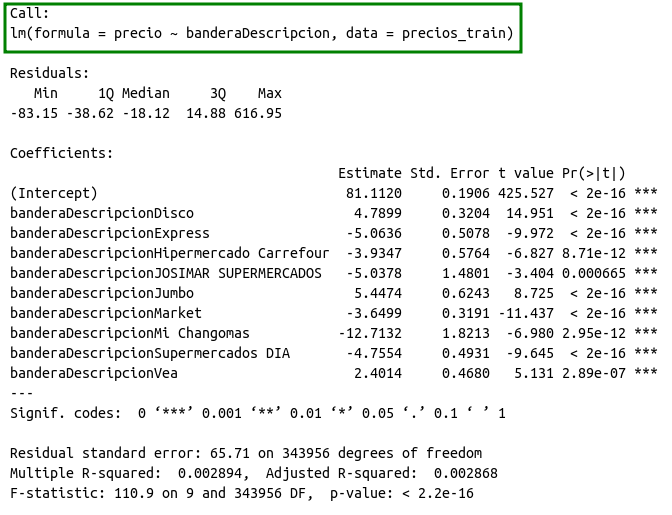
\includegraphics[scale=0.5]{img/ln_simple.png}
\end{center}

Para coparar estos dos modelos cabe destacar que en ambos casos el p-valor que se obtiene es chico, con lo cual es estadisticamente significativo en ambos casos.\\

Para el caso de precio vs banderaDescripcion:\\

Se observa que el valor del Intercept es de \$81.1504 , que se corresponde a la bandera COTO al cual si se compara con algunas de las variables dummy creadas, se puede evidenciar que el valor de Disco sobre Coto es 5.09 por ejemplo.


Para el caso de precio vs medicion:\\

Se observa que el valor del Intercept es de \$75.35 . 
Por otro lado el β1 indica por cada medicion el valor ascenderá en \$1.02, se puede concluir que el precio se forma como el valor del Intercept mas la cantidad de medicion multiplicado por \$1.02.


Comparación de modelos:\\
Para comparar estos dos modelos se utilizará el R2 Ajustado, y se evidencia que para el primer modelo el mismo tiene un valor de 0.002979 y para el segundo modelo el valor es 0.002027, por lo que se concluye que la variabilidad explicada por el primer modelo es superior a la explicada por este segundo modelo.\\
Cabe destacar que estos modelos simples son muy rudimentarios, ya que estoy queriendo explicar la variabilidad del precio solo con una variable, asi que sirven solo de punto de partida para tener una base a partir de la cual empezar a iterar en complejidad.




\subsection{Compuesto}

Para realizar una análisis mas rico para una variable precio es evidente que no basta con una sola variable, ya que el precio no es formado solamente por una de ellas sino por una conjunción de las mismas, por lo que se propone un modelo lineal compuesto donde entren en juego todas las variables que se habían definido al comienzo de la sección seleccionando las siguientes como candidatas para explicar la variabilidad de precio.\\


\begin{center}
 \begin{tabular}{||c c c c c c c||} 
 \hline
    banderaDescripcion & sucursalTipo & medicion & pVentasC & mCuadradoC \\ 
 \hline
 \hline
\end{tabular}
\end{center}


Para realizar este análisis se realizaron dos análisis por separado, uno fue un modelo lineal compuesto tradicional, y el otro logarítmico, en donde se le aplica a las variables numéricas logaritmo y se estudia la regresión para dicho set de datos transformado.
Para mayor comodidad de lectura es que se realizan los dos juntos y en los siguientes puntos se van comparando ambos modelos.\\


\subsubsection{Estudio de p-value}

Lo primero que se quiere estudiar es la significancia del modelo, y de las covariables para entender cual de ellas serán útiles para la regresión y cuales no serán significativas, para ello se realiza un análisis del p-valor para cada una de ellas:\\



\begin{figure}[H]
\makebox[\textwidth]{
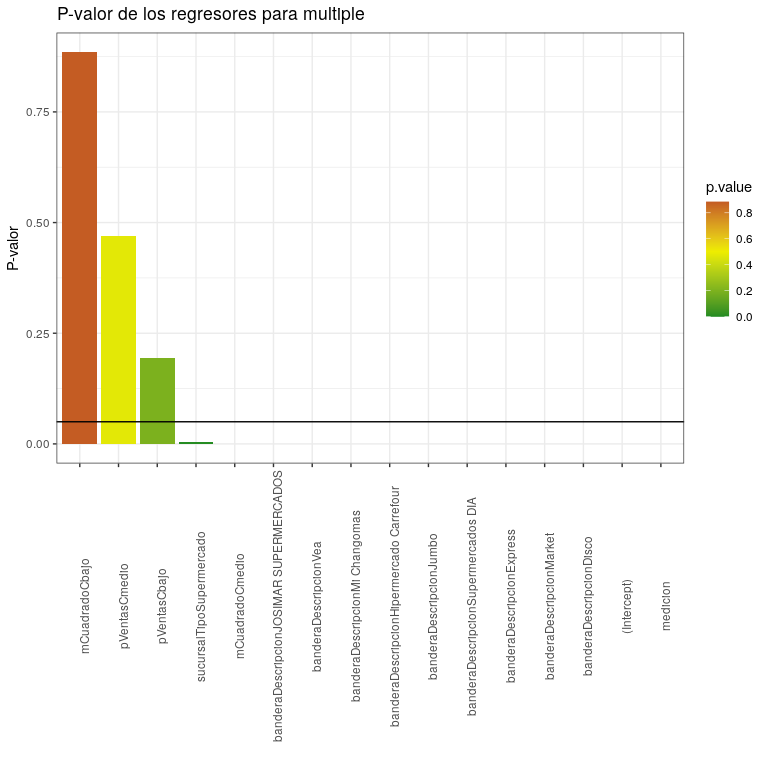
\includegraphics[width=0.4\paperwidth, height=0.4\paperheight, keepaspectratio]{img/ln_comp_pvalue.png}
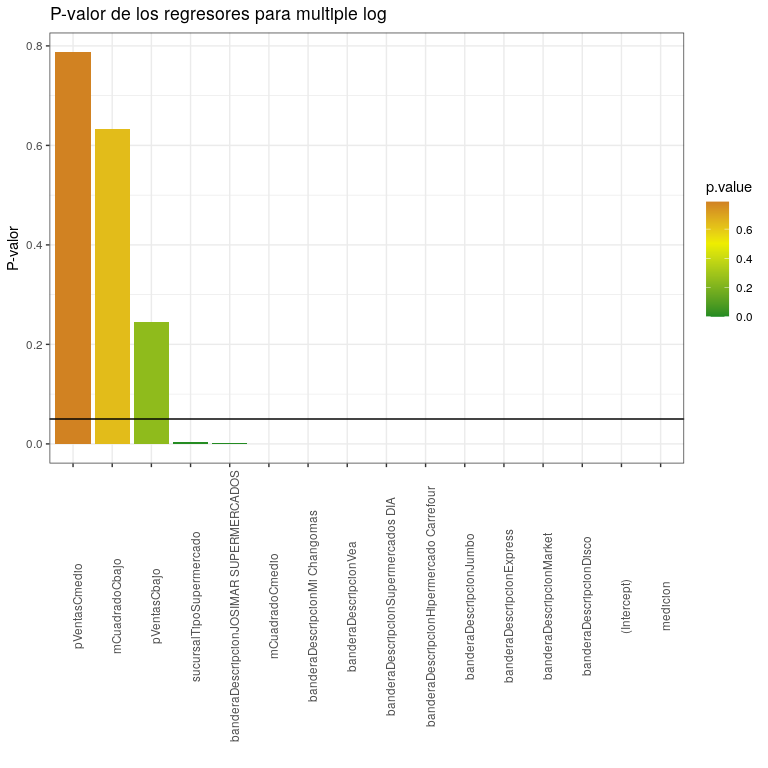
\includegraphics[width=0.4\paperwidth, height=0.4\paperheight, keepaspectratio]{img/ln_complog_pvalue.png}
}
\end{figure}



En lineas generales podemos encontrar un p-value: < 2.2e-16 para el test, pero si se miran las covariables independientemente no todas tienen un valor de significancia adecuado.
Para ambos modelos las covariables $mCuadradoCbajo$ $pVentasCmedio$ y $pVentasCbajo$ no tiene un p-value suficientemente bajo como para ser estadísticamente significativas en explicar la variabilidad de precio.\\
Cabe destacar que estas 3 variables, son parte de variables dummy que creo el modelo al generar la regresión ya que los valores de las variables orígenes eran categóricas multivaluadas.

Para completar este análisis se vuelven a comparar los coeficientes estimados y sus p-valores asociados:\\

\begin{figure}[H]
\makebox[\textwidth]{
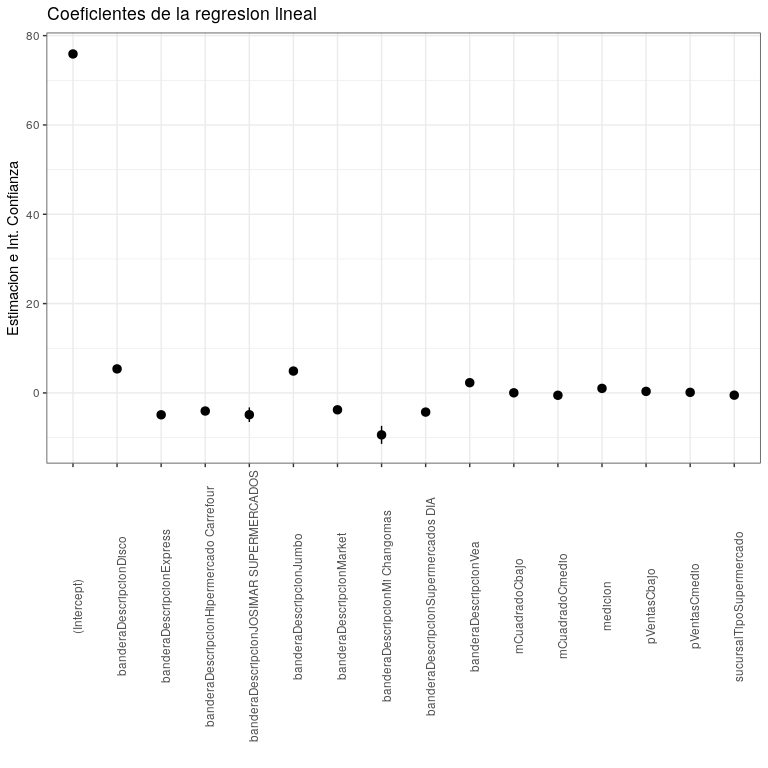
\includegraphics[width=0.4\paperwidth, height=0.4\paperheight, keepaspectratio]{img/ln_comp_coef.png}
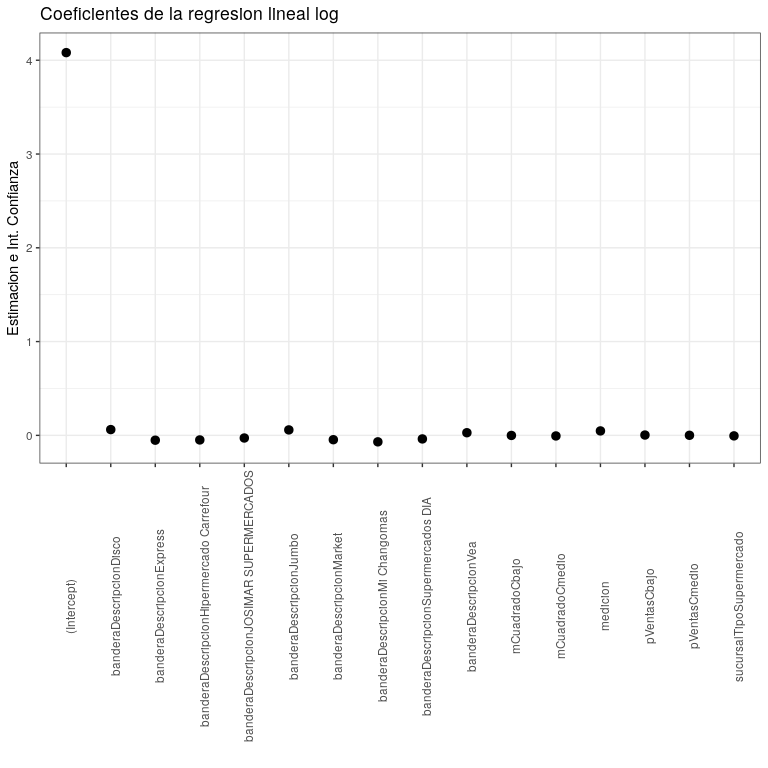
\includegraphics[width=0.4\paperwidth, height=0.4\paperheight, keepaspectratio]{img/ln_complog_coef.png}
}
\end{figure}




\subsubsection{Estudio de residuo}

Los residuos (o errores) son la diferencia entre los valores observados y los valores que predice el modelo, con lo cual se espera que estos valores sean lo mas cercano a cero posibles, a menor residuo menor es la diferencia entre lo que esta prediciendo el modelo y el valor observado.\\
Con lo cual se buscara realizar un estudio del promedio de los residuos de ambos modelos para poder compararlos:\\



\begin{center}
 \begin{tabular}{||c c||} 
 \hline
    Residuo modelo linea múltiple & Residuo modelo linea múltiple logarítmico \\ 
 \hline
 1.106236e-11 & 5.4611e-12 \\
 \hline
 \hline
\end{tabular}
\end{center}

En la siguiente comparación de gráficos podemos ver los polígonos dibujados por los residuos lo cual ayudara a entender la dispersion de los mismos:\\

\begin{figure}[H]
\makebox[\textwidth]{
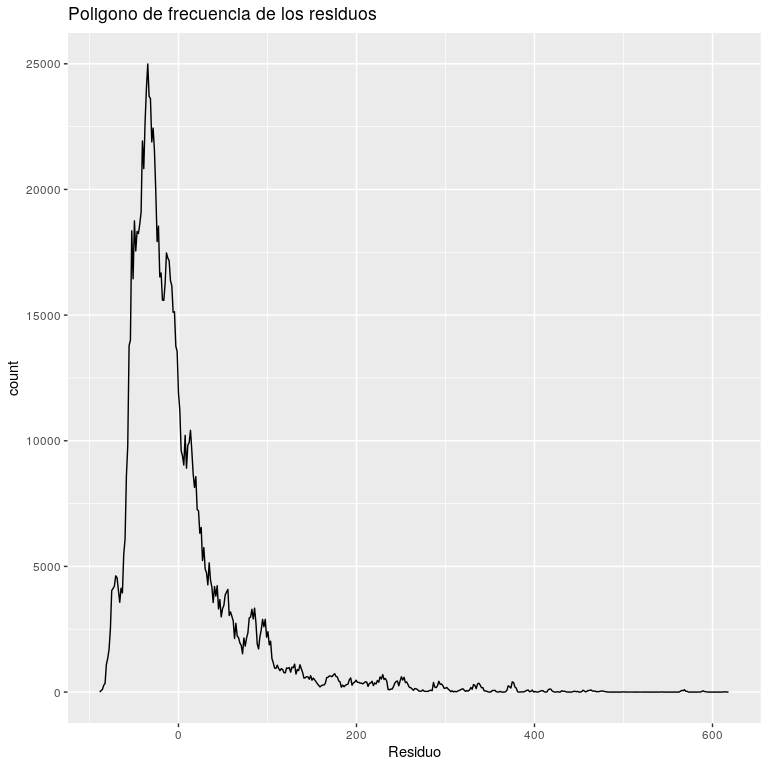
\includegraphics[width=0.4\paperwidth, height=0.4\paperheight, keepaspectratio]{img/ln_comp_poligono.png}
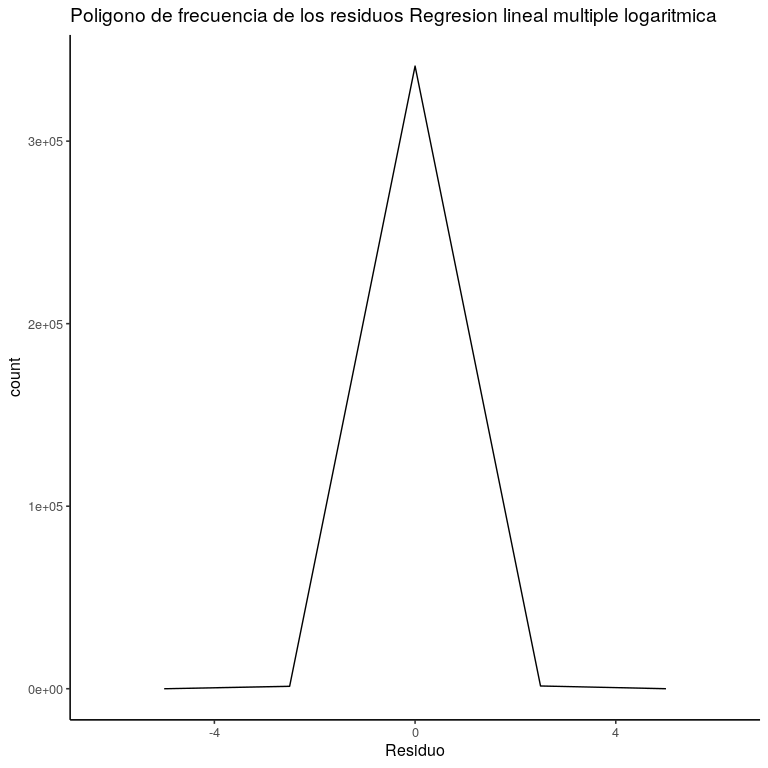
\includegraphics[width=0.4\paperwidth, height=0.4\paperheight, keepaspectratio]{img/ln_complog_poligono.png}
}
\end{figure}

Otra forma de analizar los residuos es ver si los mismos siguen una distribución teórica N(0,1), a mejor adaptación de la curva de los residuos a esta distribución mejor sera el modelo.
Luego, se grafican ambos residuos:\\



\begin{figure}[H]
\makebox[\textwidth]{
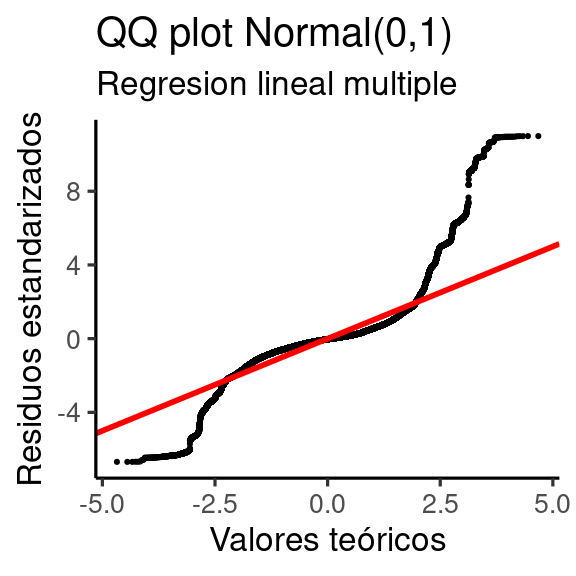
\includegraphics[width=0.4\paperwidth, height=0.4\paperheight, keepaspectratio]{img/ln_comp_qqplot.png}
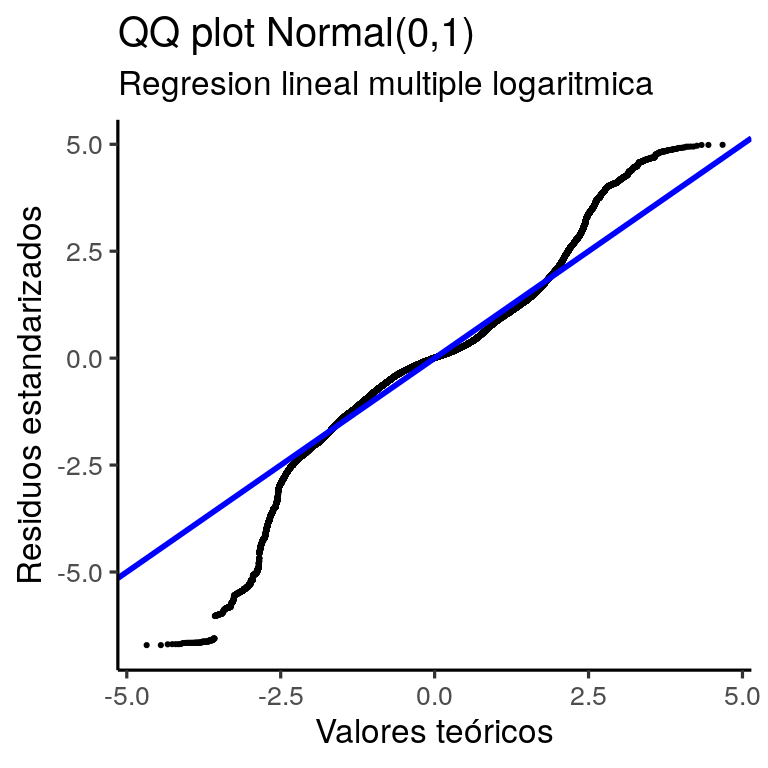
\includegraphics[width=0.4\paperwidth, height=0.4\paperheight, keepaspectratio]{img/ln_complog_qqplot.png}
}
\end{figure}



Lo que se observa en este gráfico, es que si bien en los extremos la tendencia es alejarse de la recta, los valores estan mucho mas pegados a ella que en el segundo modelo donde se aplico el logaritmo de los valores numericos, lo mismo ocurre con los valores intermedios que están prácticamente sobre la recta. \\
Por ultimo resta compara la suma de cuadrados residuales, R2 ajustados (ya que hay mas de una covariable), en la siguiente tabla se muestran los resultados obtenidos:\\


\begin{center}
 \begin{tabular}{||c c||} 
 \hline
    R2 ajustado lineal múltiple & R2 ajustado lineal múltiple logarítmico \\ 
 \hline
 0.005027542 & 0.005456552 \\
 \hline
 \hline
\end{tabular}
\end{center}

Se observa que para el caso del segundo modelo multiple, el R2 ajustado es ligeramente mas alto y por consiguiente expresando un mejor modelo.
Por todo loa anterior estudiado, se puede concluir hasta este punto que el mejor modelo es el expresado por el modelo lineal múltiple aplicando logaritmo a las variables numéricas.






\subsection{Regularización}

Las técnicas de regularización son muy útiles cuando se trabaja con un set de datos que tiene una gran cantidad de variables las cuales podrían introducir gran variabilidad a las estimaciones de los parámetros. En el caso estudiado hasta el momento si bien no hay gran cantidad de variables, se realizara un modelado con dos regresores clásicos para probar si este tipo de modelo es mejor o no para predecir el precio de los productos.\\
En esta sección se analizaran dos tipos de regresores, $Lasso$ y $Ridge$ el primero correspondiente α=1 y el segundo a α=0, se hará una comparativa entre ambos igual que antes para unificar las explicaciones y los graficos.\\
Cabe señalar que lo que diferencia entre estos métodos de regularización y los métodos lineales antes empleados, es que estas regularizaciones fuerzan a que los coeficientes de los predictores tiendan a cero. Esta penalización esta controlada por el parámetro λ. Cuando λ=0 la penalización es nula y los resultados son equivalentes a los obtenidos por mínimos cuadrados, cuando λ=infinito todos los coeficientes son cero, lo que equivale al modelo sin ningún predictor (modelo nulo).\\
La elección del parámetro λ adecuado es parte del estudio que se realizará mediante cross validation para buscar el óptimo y asi computar el modelo con el parámetro optimizado.


\subsubsection{Lasso vs Ridge}

Si bien ambos modelos son muy similares Lasso, al igual que Ridge, fuerza a que las estimaciones de los coeficientes de los predictores tiendan a cero. La diferencia es que Lasso puede fijar algunos de ellos en cero, lo que potencia la reducción de la varianza.

\subsubsection{Selección de λ}

Lo primero que se buscara es el gráfico de los coeficientes a medida que se va incrementando el valor de λ para ambos modelos:


\begin{figure}[H]
\makebox[\textwidth]{
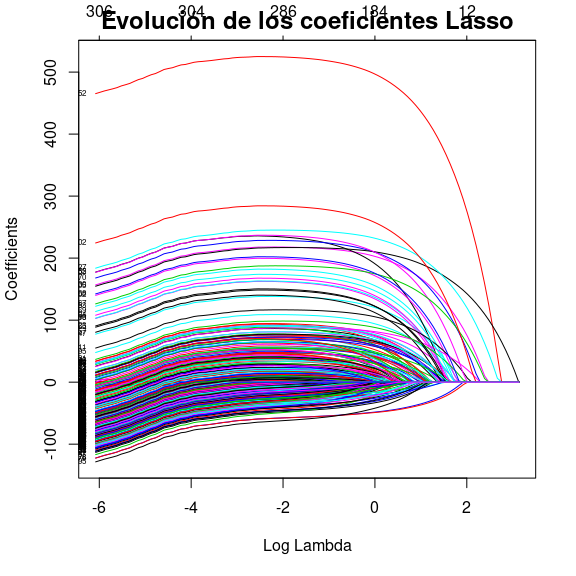
\includegraphics[width=0.4\paperwidth, height=0.4\paperheight, keepaspectratio]{img/lasso_coef.png}
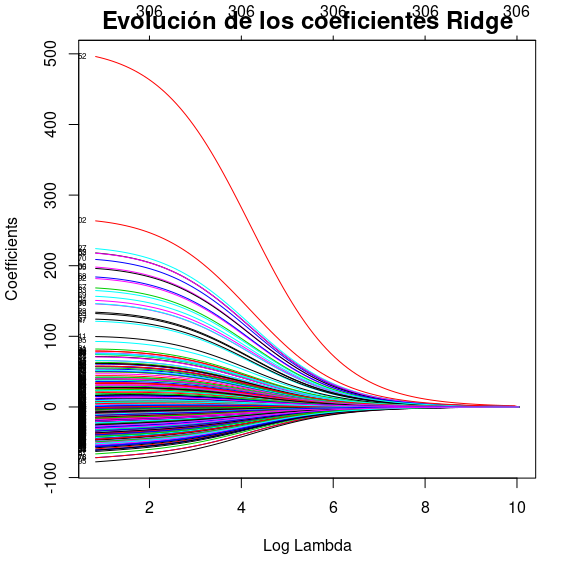
\includegraphics[width=0.4\paperwidth, height=0.4\paperheight, keepaspectratio]{img/ridge_coef.png}
}
\end{figure}

Como expresan los gráficos, los coeficientes en ambos modelos se van haciendo mas pequeños a medida que se incrementa el valor de λ.\\
Con el fin de identificar el valor de λ que da lugar al mejor modelo, se puede recurrir a Cross-Validation, en este caso utilizaremos K=5.\\



\begin{figure}[H]
\makebox[\textwidth]{
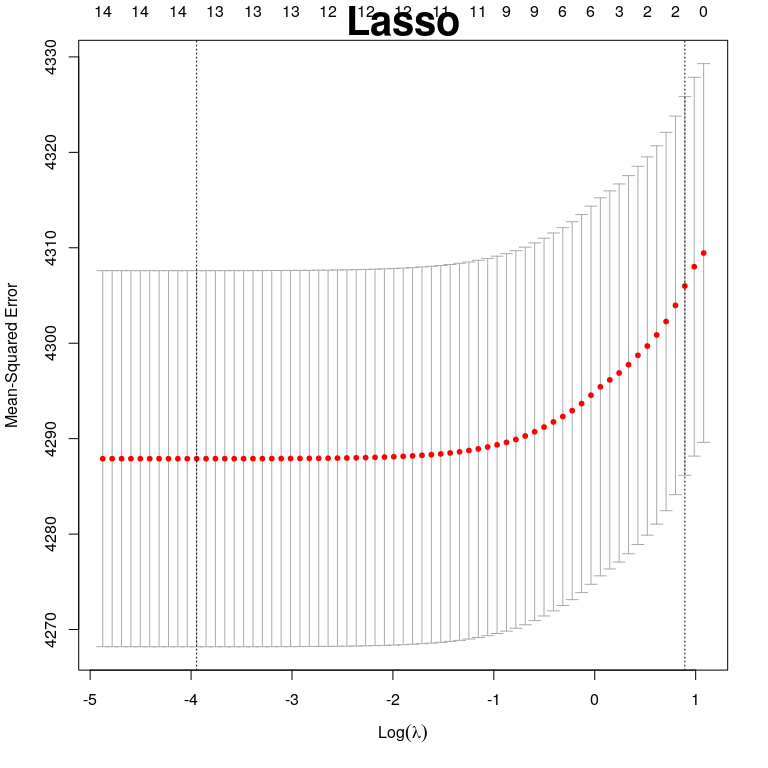
\includegraphics[width=0.4\paperwidth, height=0.4\paperheight, keepaspectratio]{img/lasso_cv.png}
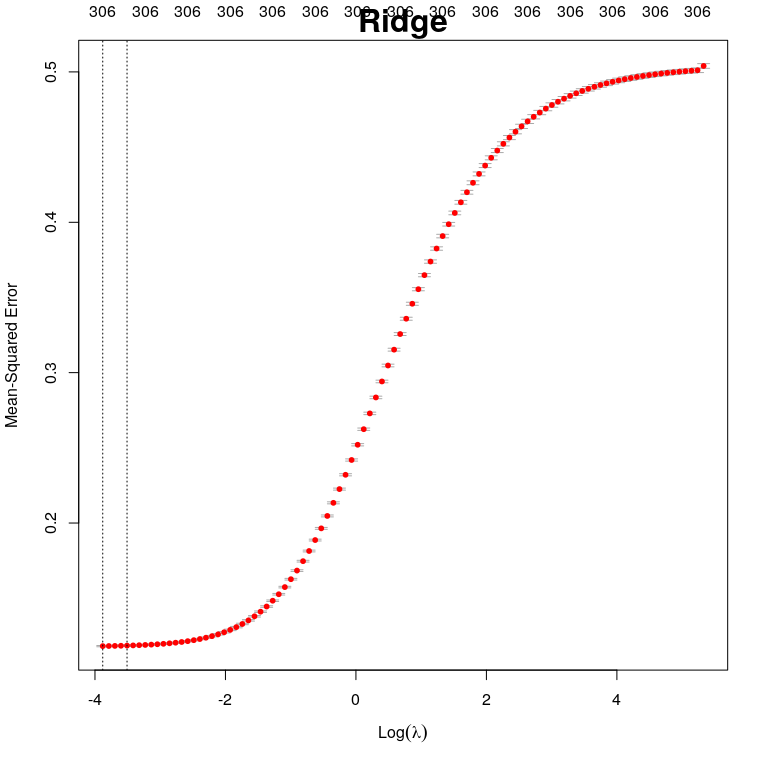
\includegraphics[width=0.4\paperwidth, height=0.4\paperheight, keepaspectratio]{img/ridge_cv.png}
}
\end{figure}


\begin{center}
 \begin{tabular}{||c c c c||} 
 \hline
    Lasso λ min & Lasso λ 1se & Ridge λ min & Ridge λ 1se  \\ 
 \hline
    0.01935577 & 2.442421 & 0.01935577 & 2.442421\\
 \hline
 \hline
\end{tabular}
\end{center}


Los gráficos muestran el MSE (Mean Square Error) para cada valor de λ junto con la barra de error correspondiente. Se marcan dos valores de λ específicos, el valor con el que se consigue el menor error y el valor con el que se consigue el modelo mas sencillo que se aleja a menos de 1 de desvío estandar del mínimo MSE posible. \\
También el gráfico evidencia la media del MSE con su limite superior e inferior y la cantidad de variables que sobreviven para cada valor de lambda.\\
Se volverá a correr los modelos pero esta ves con los valores min de λ óptimos calculados.\\

Se realiza un calculo de ambos modelos para el valor de R2 y Root Mean Square Error (RMSE) para ambos modelos:


\begin{center}
 \begin{tabular}{||c c c c||} 
 \hline
    Lasso R2 & Lasso RMSE & Ridge R2 & Ridge RMSE  \\ 
 \hline
    0.005039739 & 65.481091 & 0.005040342 & 65.48107\\
 \hline
 \hline
\end{tabular}
\end{center}


\subsection{Comparación de Modelos}

Identificar el mejor método para un problema en particular consiste en dividir las observaciones disponibles en dos grupos (trainig (70\%) y test(30\%)). Luego se ajusto el modelo únicamente con el training y se calcula el MSE \left(Promedio\left(predicción - valor real\right)^{2}\right) utilizando el test set.\\

De los métodos, el que obtiene el menor MSE es el que obtuvo las predicciones mas cercanas a los valores observados, con lo cual el mejor.










